\chapter{Fundamental Identity, Ray Structure, and Universal Parametrisation}
\label{sec:visualisierung}

% ─────────────────────────────────────────────────────────────────────────────
\section{Equidistant Parametrisation of the Spiral}
% ─────────────────────────────────────────────────────────────────────────────

On the Archimedean spiral $r(\theta) = \tfrac{6}{\pi^2}\,\theta$,
points are to be placed that follow one another at \emph{constant
arc-length spacing} $\Delta s = 1$. This equidistant parametrisation
leads to a characteristic geometric scaling factor.

\subsection{Derivation of the Scaling Factor \texorpdfstring{$\sqrt{3}$}{sqrt(3)}}

The arc length of the spiral from $0$ to $\theta$ is:
\[
  s(\theta)
  = \frac{a}{2}\!\left[\theta\sqrt{\theta^2+1}
    + \operatorname{arcsinh}(\theta)\right],
  \qquad a = \frac{6}{\pi^2}.
\]
For large $\theta$ the quadratic term dominates:
\[
  s(\theta) \;\approx\; \frac{a}{2}\,\theta^2
           \;=\; \frac{3}{\pi^2}\,\theta^2.
\]
For the $k$-th point to lie at $s_k = k$ (unit spacing), we require:
\[
  \frac{3}{\pi^2}\,\theta_k^2 = k
  \;\;\implies\;\;
  \theta_k = \frac{\pi}{\sqrt{3}}\,\sqrt{k}.
\]
The angle thus grows with the \emph{square root} of the index $k$, and the
\textbf{scaling factor $\sqrt{3}$} arises directly from the
geometry of the spiral as a consequence of the condition $\Delta s = 1$.

The corresponding radial coordinate:
\[
  r_k
  = \frac{6}{\pi^2}\cdot\theta_k
  = \frac{6}{\pi^2}\cdot\frac{\pi\sqrt{k}}{\sqrt{3}}
  = \frac{6\sqrt{k}}{\pi\sqrt{3}}
  = \frac{2\sqrt{3k}}{\pi}.
\]

\begin{table}[H]
\centering
\renewcommand{\arraystretch}{1.2}
\caption{Actual arc-length spacing $\Delta s$ between
  consecutive equidistant points---convergence towards $1$.}
\begin{tabular}{cccc}
\toprule
$k$ & $\theta_k = \pi\sqrt{k}/\sqrt{3}$ & $r_k = 2\sqrt{3k}/\pi$ & $\Delta s_k \to 1$ \\
\midrule
   10 &   5.7357 &   3.4869 & 1.01589 \\
  100 &  18.1380 &  11.0266 & 1.00153 \\
 1000 &  57.3574 &  34.8691 & 1.00015 \\
10000 & 181.3799 & 110.2658 & 1.00002 \\
\bottomrule
\end{tabular}
\end{table}

% ─────────────────────────────────────────────────────────────────────────────
\section{\texorpdfstring{$\sqrt{3}$}{sqrt(3)} as the Common Scaling Factor of \texorpdfstring{$k(n)$}{k(n)} and the Spiral}
% ─────────────────────────────────────────────────────────────────────────────

The scaling factor $\sqrt{3}$ of the equidistant
construction simultaneously appears as the \emph{stretching factor of
the quadratic sequence} $k(n)$. This dual nature of $\sqrt{3}$
reveals a shared structural character of both structures.

\subsection{Step 1 --- Leading Coefficient of \texorpdfstring{$k(n)$}{k(n)}}

The sequence $k(n) = \tfrac{1}{6}(2n^2 + 3n + 1)$ has the leading term:
\[
  k(n) = \frac{1}{3}\,n^2 + \frac{1}{2}\,n + \frac{1}{6}.
\]
The stretching factor of the parabola is $\tfrac{1}{3} = \tfrac{1}{(\sqrt{3})^2}$:
the factor $\sqrt{3}$ appears in the denominator of the quadratic coefficient.

\subsection{Step 2 --- Stretching Factor of the Arc Length}

The asymptotic arc length of the spiral reads:
\[
  s(\theta) \approx \frac{3}{\pi^2}\,\theta^2.
\]
Here the numerator carries the factor $3 = (\sqrt{3})^2$---precisely the
reciprocal of the parabola coefficient.

\begin{tcolorbox}[
  colback=blue!3, colframe=blue!40!black, enhanced,
  title={Reciprocal Relationship of the Stretching Factors}]
\[
  \underbrace{\frac{1}{3}}_{\text{Parabola coeff.\ in }k(n)}
  \;\cdot\;
  \underbrace{3}_{\text{Arc-length coeff.\ of the spiral}}
  \;=\; 1.
\]
Both structures carry the same factor $\sqrt{3}$, but in
\emph{reciprocal roles}: the parabola stretches by $1/(\sqrt{3})^2$,
the spiral by $(\sqrt{3})^2$.
\end{tcolorbox}

\subsection{Step 3 --- \texorpdfstring{$\theta_{k(n)} = \theta_n$}{Angular Agreement} (asymptotically)}

Substituting $k = k(n)$ into the equidistant angular formula and
expanding $\sqrt{k(n)}$ via Taylor:
\begin{align*}
  \sqrt{k(n)}
  &= \sqrt{\frac{n^2}{3} + \frac{n}{2} + \frac{1}{6}}
   = \frac{n}{\sqrt{3}}\sqrt{1 + \frac{3}{2n} + \frac{1}{2n^2}} \\
  &\approx \frac{n}{\sqrt{3}}\!\left(1 + \frac{3}{4n}\right)
   = \frac{n}{\sqrt{3}} + \frac{3}{4\sqrt{3}}.
\end{align*}

This yields the equidistant angle at the position $k = k(n)$:
\[
  \theta_{k(n)}
  = \frac{\pi}{\sqrt{3}}\cdot\sqrt{k(n)}
  \approx \frac{\pi}{\sqrt{3}}\!\left(\frac{n}{\sqrt{3}} + \frac{3}{4\sqrt{3}}\right)
  = \frac{\pi n}{3} + \frac{3\pi}{4 \cdot 3}
  = \frac{\pi n}{3} + \frac{\pi}{4}.
\]

This is the actual helix angle $\theta_n = \tfrac{\pi}{3}n + \tfrac{\pi}{4}$:

\begin{satz}[\texorpdfstring{$\sqrt{3}$}{sqrt(3)}-Invariance]\label{satz:sqrt3}
The equidistant spiral parametrisation, evaluated at the
positions $k = k(n)$, approximately reproduces the helix angles:
\[
  \theta_{k(n)}
  = \frac{\pi}{\sqrt{3}}\,\sqrt{k(n)}
  \approx \frac{\pi}{3}\,n + \frac{\pi}{4}
  = \theta_n.
\]
The error is of order $O(1/n)$ and converges to~$0$.
\end{satz}

\begin{table}[H]
\centering
\renewcommand{\arraystretch}{1.2}
\caption{Comparison of $\theta_{k(n)}$ (equidistant, asymptotic) and $\theta_n$ (helix)---the difference converges to~$0$.}
\begin{tabular}{ccccc}
\toprule
$n$ & $k(n)$ & $\theta_{k(n)}$ & $\theta_n = \frac{\pi n}{3}+\frac{\pi}{4}$ & Difference \\
\midrule
 5  &  11  &  6.015692 &  6.021386 & $-$0.005694 \\
11  &  46  & 12.301786 & 12.304571 & $-$0.002785 \\
19  & 130  & 20.680495 & 20.682152 & $-$0.001657 \\
47  & 760  & 50.002998 & 50.003683 & $-$0.000685 \\
97  & 3185 & 102.363226 & 102.363561 & $-$0.000335 \\
\bottomrule
\end{tabular}
\end{table}

\begin{bemerkung}[Geometric Interpretation]
The statement $\theta_{k(n)} \approx \theta_n$ means: if one places
equidistant points with unit spacing on the Archimedean spiral
and accesses them via the index $k = k(n)$, one arrives approximately
at exactly the same angles as the integer points of the helix.
The sequence $k(n)$ is \emph{the indexing induced by the common factor $\sqrt{3}$}
of the equidistant spiral parametrisation through the common
scaling factor $\sqrt{3}$.
\end{bemerkung}

% ─────────────────────────────────────────────────────────────────────────────
\section{Three Equivalent Representations in Desmos}
% ─────────────────────────────────────────────────────────────────────────────

The same equidistant parametrisation can be expressed in
Desmos~\cite{Desmos2024} through different formulae. Depending on the
chosen form, the slider parameter $h$ takes a different numerical value,
even though all three versions generate \emph{identical points} on the spiral:

\begin{table}[H]
\centering
\renewcommand{\arraystretch}{1.4}
\caption{Three equivalent formula versions for the equidistant parametrisation.
  All produce exactly the same points at unit spacing $\Delta s=1$.}
\begin{tabular}{clcl}
\toprule
Form & Formula $\theta_k$ & $h$ for $\Delta s=1$ & Occurrence \\
\midrule
A & $\dfrac{\pi\sqrt{k}}{\sqrt{3}}$
  & $\sqrt{3} \approx 1.732$
  & Project standard {\small(\texttt{Power\_equidistant\_Spiral\_v6})} \\[8pt]
B & $\dfrac{2\pi\sqrt{k}}{h}$
  & $2\sqrt{3} \approx 3.464$
  & {\small\texttt{equidistant\_Spiral\_v5}} \\[8pt]
C & $\dfrac{\pi\sqrt{3k}}{h}$
  & $3$
  & Alternative notation \\
\bottomrule
\end{tabular}
\end{table}

\begin{bemerkung}[Why Three Different $h$-Values?]
The three forms arise from algebraic rearrangement of the same expression:
\[
  \underbrace{\frac{\pi\sqrt{k}}{\sqrt{3}}}_{\text{Form A}}
  \;=\; \underbrace{\frac{2\pi\sqrt{k}}{2\sqrt{3}}}_{\text{Form B}}
  \;=\; \underbrace{\frac{\pi\sqrt{3k}}{3}}_{\text{Form C}}.
\]
The project uses \textbf{Form~A} with the derived scaling factor
$\sqrt{3}$, since this emerges directly from the derivation. The
simplified representation $h = \sqrt{3}$ is thus the geometrically
motivated constant of the spiral.
\end{bemerkung}

% ─────────────────────────────────────────────────────────────────────────────
\section{Ray Structure as a Function of the Formula Term}
% ─────────────────────────────────────────────────────────────────────────────

The following comparison shows how the visual impression of the
spiral depends on the choice of the $h$-parameter in Form~B. The
slider parameter $h$ changes the angular spacing between the
placed points and thus the pattern of visible diagonals
(parastichies).

\begin{center}
\begin{minipage}[t]{0.65\textwidth}
  \centering
  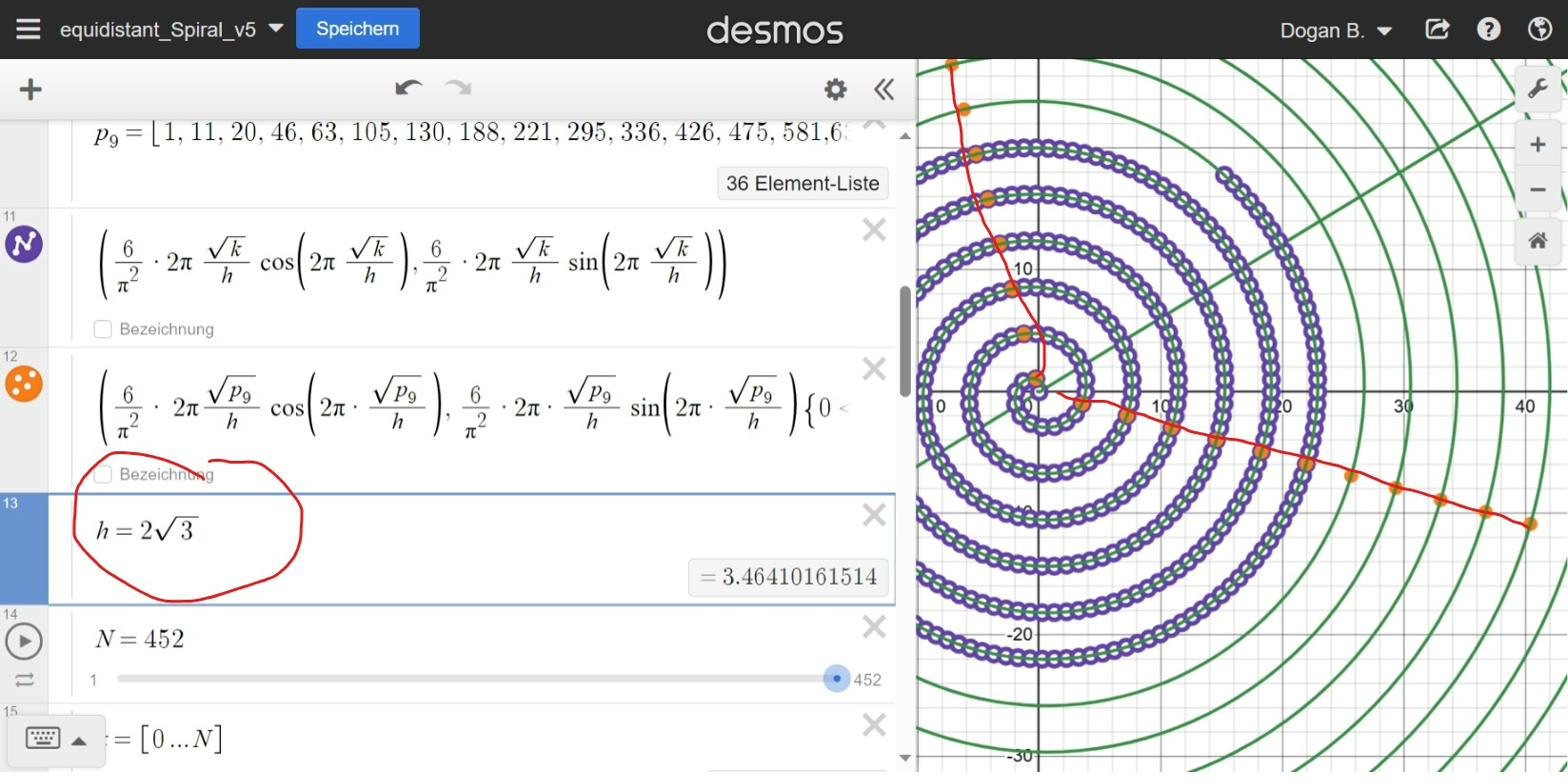
\includegraphics[width=\textwidth]{bilder/h_2sqrt3_strahlen}\\[4pt]
  \small\textbf{$h = 2\sqrt{3}$ (Form B)} \\[2pt]
  \small \textbf{Project standard}: corresponds to $h_A = \sqrt{3}$ in Form A.\\
  \small Arc-length spacing $\Delta s \approx 1$, uniform point distribution.
\end{minipage}
\end{center}

\vspace{1.4cm}

\noindent
\begin{minipage}[t]{0.47\textwidth}
  \centering
  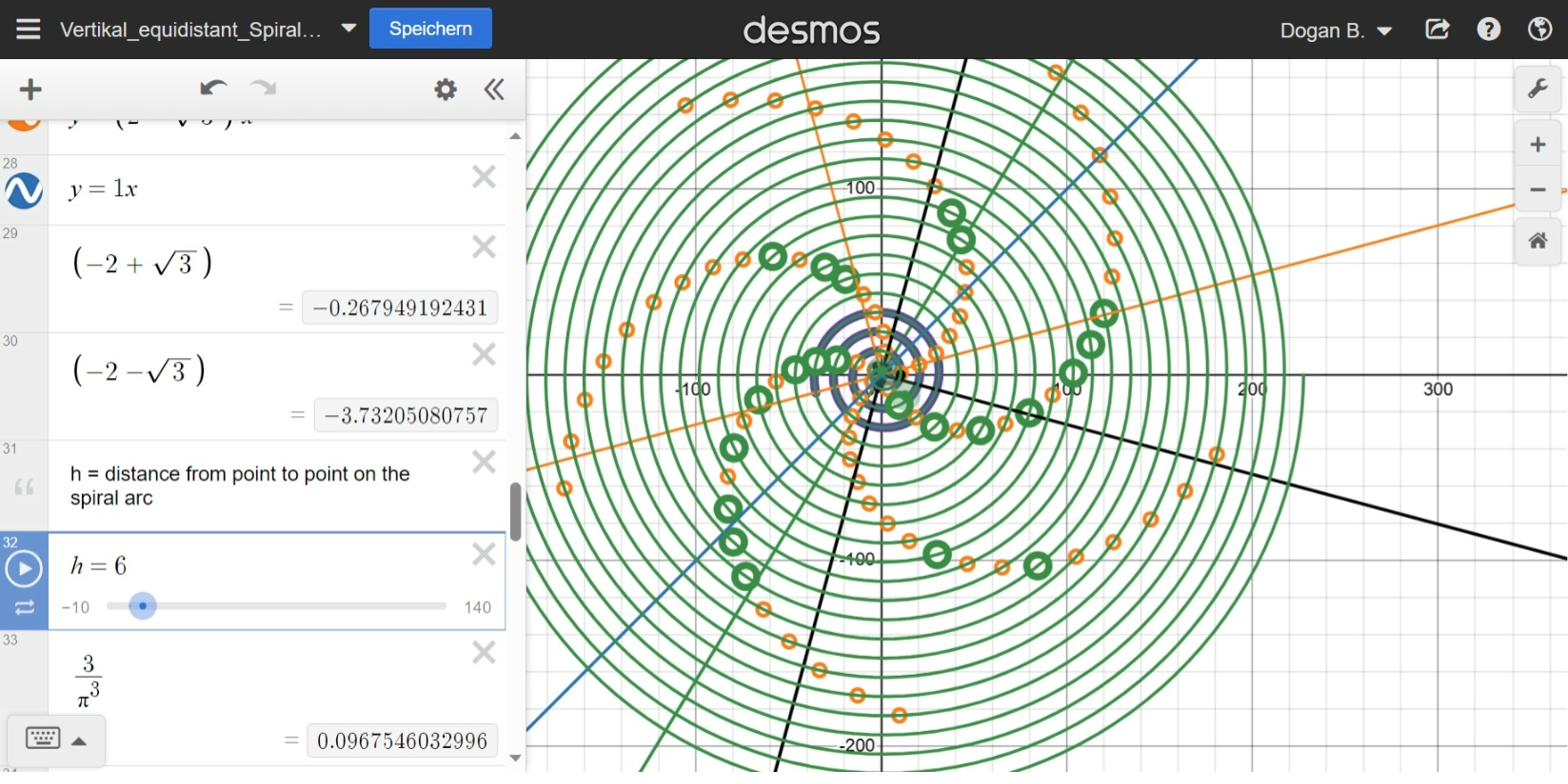
\includegraphics[width=\textwidth]{bilder/h6_strahlen}\\[4pt]
  \small\textbf{$h = 6$ (Form B)} \\[2pt]
  \small Corresponds to $h_A = 3$ in Form A. \\
  \small Arc-length spacing $\Delta s \approx 1/3$.\\
  \small Integer density distributes over 5 parastichy arms.
\end{minipage}
\hfill
\begin{minipage}[t]{0.47\textwidth}
  \centering
  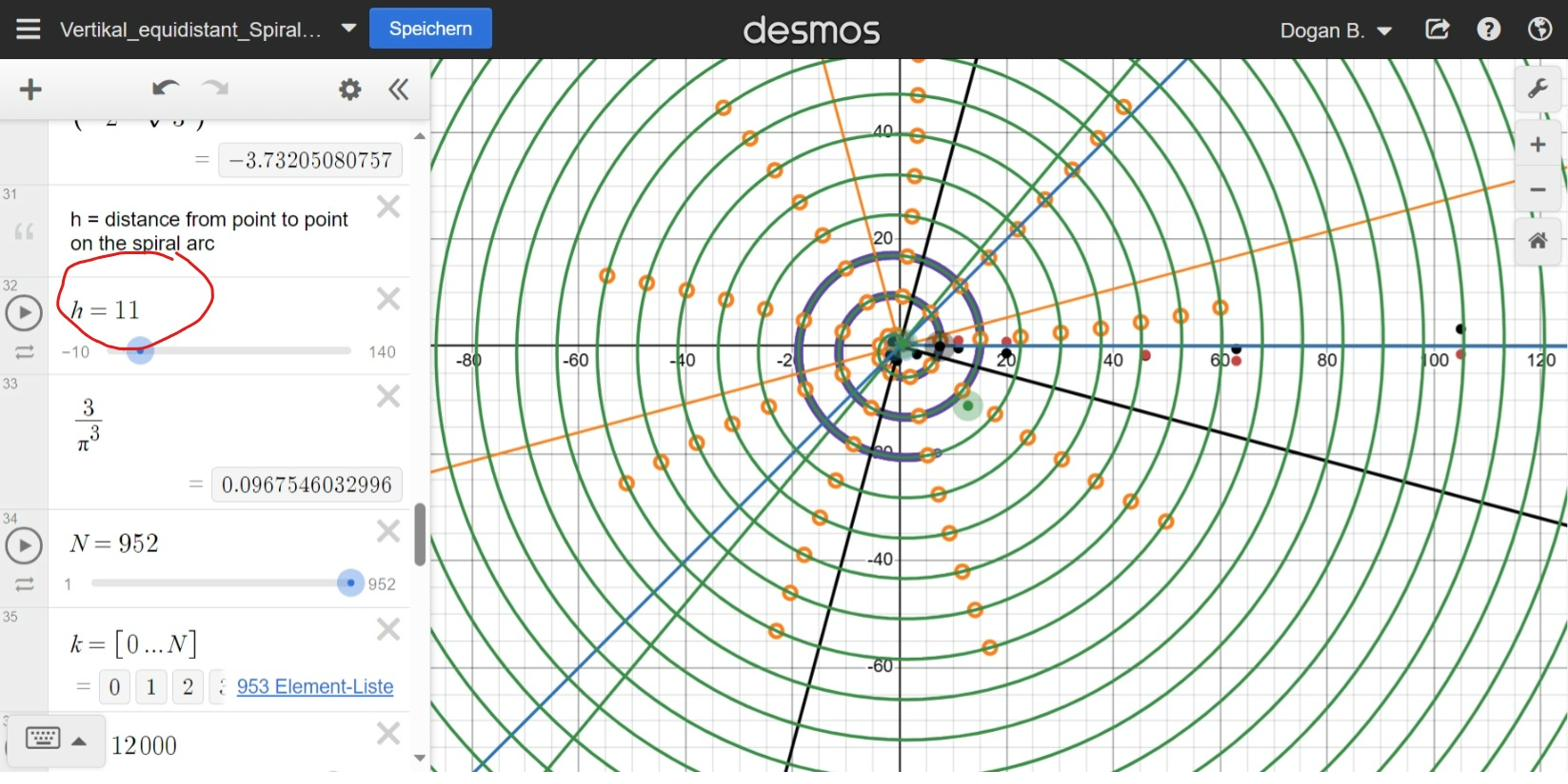
\includegraphics[width=\textwidth]{bilder/h11_strahlen}\\[4pt]
  \small\textbf{$h = 11$ (Form B)} \\[2pt]
  \small Arc-length spacing $\Delta s \approx 12/121 \approx 0.1$.\\
  \small Expansive diagonal structure. Integers distribute over 9 lines.
\end{minipage}

\vspace{1.0cm}

\begin{center}
\small\textit{All four representations show the same Archimedean spiral
$r = \tfrac{6}{\pi^2}\theta$ (Desmos, $N \approx 952$ points).
The slider parameter $h$ follows Formula~B: $\theta_k = 2\pi\sqrt{k}/h$.
The project standard $h_A = \sqrt{3}$ (Form~A) corresponds to $h_B = 2\sqrt{3}$
in these images. The circle markers correspond to the sequence values $k(n)$;
the coloured diagonals run along the residue classes
$n \equiv 1,5 \pmod{6}$.}
\end{center}

% ─────────────────────────────────────────────────────────────────────────────
\section{Direct Derivation of the Height Function from the Quadratic Sequence}
\label{sec:hoehenherleitung}
% ─────────────────────────────────────────────────────────────────────────────

\subsection{Two Paths --- One Statement: Why Both Derivations Are Valuable}

In the preceding section, the helix angle $\theta_n$ was obtained
through a Taylor expansion of $\sqrt{k(n)}$ \emph{asymptotically}
(Theorem~\ref{satz:sqrt3}). This approach is deliberately preserved
as an independent method---for it works for \emph{arbitrary
quadratic polynomials}, without presupposing the specific arithmetic
structure of $k(n)$. This makes it a general tool for other researchers.

\begin{tcolorbox}[
  colback=green!4, colframe=green!40!black, enhanced,
  title={Methodological Note for Other Polynomials}]
For an arbitrary quadratic sequence $p(n) = an^2 + bn + c$, the
asymptotic procedure applies analogously:
\[
  \sqrt{p(n)} \approx \sqrt{a}\,n + \frac{b}{2\sqrt{a}},
\]
from which the spiral angle grows linearly in $n$; its slope $\sqrt{2a/A}$ is determined jointly by the leading coefficient $a$ and the slope $A$ of the associated spiral (for $k(n)$: $\pi/3$). The approximation method requires only knowledge of the
leading coefficient---\emph{no} completing the square and \emph{no}
integrality property. It is therefore applicable to a substantially
broader class of sequences.

The exact method (following section) requires instead that
$\deg(p) \cdot \text{(prefactor)} \cdot p(n) + 1$ be a perfect
square---a property that $k(n) = \tfrac{1}{6}(2n^2+3n+1)$
happens to possess, but most polynomials do not.
\end{tcolorbox}

In the following it is shown that for $k(n)$ itself an \emph{exact}
derivation is possible---without approximation and with complete
error resolution. The key is the invertibility of $k(n)$
and a hidden perfect-square property.

% ─────────────────────────────────────────────────────────────────────────────
\subsection{The Sequence \texorpdfstring{$k(n)$}{k(n)} and Its Exact Inverse}
\label{subsec:inverse}
% ─────────────────────────────────────────────────────────────────────────────

The starting point is the quadratic sequence
\begin{equation}\label{eq:k_def}
  k(n) = \frac{2n^2 + 3n + 1}{6} = \frac{(n+1)(2n+1)}{6},
  \qquad n \equiv 1, 5 \pmod{6}.
\end{equation}
This formula assigns to each index $n$ (the helix height) a
spiral index $k$. The question is: What is the
\emph{inverse function}---that is, $n$ as a function of $k$?

The naive answer via the quadratic formula yields:
\begin{equation}\label{eq:lsg_formel}
  2n^2 + 3n + 1 = 6k
  \;\implies\;
  n = \frac{-3 + \sqrt{9 - 8(1-6k)}}{4}
    = \frac{-3 + \sqrt{48k + 1}}{4}.
\end{equation}
This is an \emph{exact} formula---but it contains a square root
that is irrational for general $k$. The key identity:
at the integer positions $k = k(n)$ this square root is always
an integer.

\subsection{Fundamental Identity: The \texorpdfstring{$(4n+3)^2$}{(4n+3)^2} Relation}
\label{subsec:fundamentale_identitaet}

\begin{satz}[Fundamental Identity]\label{satz:fundamental}
For all $n \geq 0$ the following holds exactly:
\begin{equation}\label{eq:fundamental}
  \boxed{(4n+3)^2 = 48\,k(n) + 1.}
\end{equation}
\end{satz}

\begin{proof}
Direct substitution of~\eqref{eq:k_def}:
\[
  48\,k(n) + 1
  = 48\cdot\frac{2n^2 + 3n + 1}{6} + 1
  = 8(2n^2 + 3n + 1) + 1
  = 16n^2 + 24n + 9
  = (4n+3)^2. \qedhere
\]
\end{proof}

\noindent
The identity explains why formula~\eqref{eq:lsg_formel}
yields integer values at the positions $k = k(n)$: the polynomial $k(n)$
is constructed so that $48k(n)+1$ is always a perfect square,
namely $(4n+3)^2$.

\begin{bemerkung}[The Derivative as a Bridge]
The derivative $k'(n) = (4n+3)/6$ exhibits the same expression $4n+3$.
Identity~\eqref{eq:fundamental} can therefore also be written as:
\[
  \bigl[6\,k'(n)\bigr]^2 = 48\,k(n) + 1,
\]
i.e., the growth rate of the sequence and its value are linked by an exact
algebraic relation---a property that does \emph{not} hold for general
quadratic polynomials.
\end{bemerkung}

% ─────────────────────────────────────────────────────────────────────────────
\subsection{Exact Inverse Formula: Height from Spiral Index}
\label{subsec:umkehrformel}
% ─────────────────────────────────────────────────────────────────────────────

From Theorem~\ref{satz:fundamental} the exact inverse of $k(n)$
follows immediately.

\begin{satz}[Exact Height Function]\label{satz:hoehenfunktion}
The unique non-negative solution of the equation $k(n) = k$ is:
\begin{equation}\label{eq:n_von_k}
  \boxed{n(k) = \frac{\sqrt{48k + 1} - 3}{4}.}
\end{equation}
This is the exact height function of the helix: $z(k) = n(k)$.
\end{satz}

\begin{proof}
From $(4n+3)^2 = 48k+1$ it follows that $4n+3 = \sqrt{48k+1}$ (since $4n+3 > 0$),
hence $n = (\sqrt{48k+1}-3)/4$.
\end{proof}

\begin{bemerkung}[Comparison: Asymptotic vs.\ Exact]
\label{bem:vergleich}
The asymptotic approximation from the previous section reads
$n \approx \sqrt{3k} - 3/4$. Comparison with the exact formula
makes the difference visible and quantifies the error:
\begin{align*}
  n_{\mathrm{exact}}(k)
  &= \frac{\sqrt{48k+1}-3}{4}
   = \frac{4\sqrt{3k}\sqrt{1+\frac{1}{48k}}-3}{4}
   = \sqrt{3k}\underbrace{\sqrt{1+\frac{1}{48k}}}_{\approx\,1+\frac{1}{96k}}
     - \frac{3}{4} \\
  &= \sqrt{3k} + \underbrace{\frac{\sqrt{3}}{96\sqrt{k}}}_{\text{correction term}}
     - \frac{3}{4}, \\[6pt]
  n_{\mathrm{asympt.}}(k)
  &= \sqrt{3k} - \frac{3}{4}.
\end{align*}
The absolute error of the approximation is $+\tfrac{\sqrt{3}}{96\sqrt{k}}$
and is always \emph{positive}: the asymptotic formula systematically
underestimates the true value $n$. For $k = k(n)$ this error is of
order $O(n^{-1})$.
\end{bemerkung}

% ─────────────────────────────────────────────────────────────────────────────
\subsection{The Universal Quantity \texorpdfstring{$Q(k)$}{Q(k)}: All Helix Quantities from a Single Root}
\label{subsec:Q}
% ─────────────────────────────────────────────────────────────────────────────

The fundamental identity~\eqref{eq:fundamental} raises the question whether all previously derived geometric quantities can be expressed through a single scalar. The identity suggests treating the expression under the square root as exactly this quantity:
\begin{equation}\label{eq:Q_def}
  Q(k) \coloneqq \sqrt{48k + 1}.
\end{equation}

Universality is meant construction-internally: every geometric quantity
of the helix developed in this work --- index, angle, radius,
circumference, apex height, generator length, asymptotic torsion --- is
an explicit function of $Q$ alone, as the following table shows; no
universality beyond this construction is claimed.

At the lattice points $k = k(n)$, $Q$ always takes the integer
value $Q(k(n)) = 4n+3$. Thus $Q$ becomes the universal
bridge between the spiral index $k$ and all geometric quantities of the helix.

\begin{table}[H]
\centering
\renewcommand{\arraystretch}{1.45}
\caption{All geometric characteristics of the helix as exact functions
  of $Q(k) = \sqrt{48k+1}$. At the lattice points $k = k(n)$,
  $Q = 4n+3$ (integer); the third column gives the
  value there directly.}
\begin{tabular}{llll}
\toprule
Characteristic & Exact formula in $Q$ & Value at $k=k(n)$ & Unit \\
\midrule
Height (inverse of $k$)    & $z = \dfrac{Q-3}{4}$
    & $n$
    & --- \\[8pt]
Height above apex          & $h = \dfrac{Q}{4}$\\[8pt]
Radius (cone)              & $r = \dfrac{Q}{2\pi}$
    & $\dfrac{4n+3}{2\pi}$
    & --- \\[8pt]
Azimuthal angle (spiral)   & $\theta = \dfrac{\pi Q}{12}$
    & $\dfrac{\pi}{3}n+\dfrac{\pi}{4}$
    & rad \\[8pt]
Derivative $k'(n)$         & $k' = \dfrac{Q}{6}$
    & $\dfrac{4n+3}{6}$
    & --- \\[8pt]
Generator length           & $\ell = \dfrac{Q}{2\pi}\sqrt{1+\tfrac{\pi^2}{4}}$
    & $r_n\,|\vec{v}|$
    & --- \\[8pt]
\bottomrule
\end{tabular}
\label{tab:Q_uebersicht}
\end{table}

\noindent
The table makes visible what the asymptotic method captures only
\emph{approximately}: the helix is completely determined by the
\emph{single} function $Q(k) = \sqrt{48k+1}$. The
asymptotic formula used in Chapter~\ref{sec:visualisierung},
$\theta \approx (\pi/\sqrt{3})\sqrt{k}$, is nothing other than
the leading approximation of $\theta = \pi Q / 12 \approx \pi \cdot 4\sqrt{3k}/12
= (\pi/\sqrt{3})\sqrt{k}$ for large $k$.

% ─────────────────────────────────────────────────────────────────────────────
\subsection{Verification of the Cone and Spiral Equations (Exact)}
\label{subsec:verifikation}
% ─────────────────────────────────────────────────────────────────────────────

Both core geometric statements---cone conformity and spiral conformity---hold
exactly with the $Q$-representation, not merely asymptotically.

\begin{satz}[Cone Conformity]\label{satz:kegel}
The helix points $(r(k),\, z(k))$ lie exactly on the cone
$z = -\tfrac{3}{4} + \tfrac{\pi}{2}\,r$:
\[
  -\frac{3}{4} + \frac{\pi}{2}\cdot\frac{Q}{2\pi}
  = -\frac{3}{4} + \frac{Q}{4}
  = \frac{Q-3}{4}
  = z(k). \qquad \square
\]
\end{satz}

\begin{satz}[Spiral Conformity]\label{satz:spirale}
The helix points $(r(k),\, \theta(k))$ lie exactly on the
Archimedean spiral $r = \tfrac{6}{\pi^2}\,\theta$:
\[
  \frac{6}{\pi^2}\cdot\frac{\pi Q}{12}
  = \frac{Q}{2\pi}
  = r(k). \qquad \square
\]
\end{satz}

\noindent
In both cases every approximation vanishes: the identities are
algebraic consequences of the structure of $k(n)$ and hold for
all $k$, not only for $k \to \infty$.

% ─────────────────────────────────────────────────────────────────────────────
\subsection{ODE Characterisation of the Height Function}
\label{subsec:ode}
% ─────────────────────────────────────────────────────────────────────────────

The exact formula~\eqref{eq:n_von_k} possesses a direct
interpretation as the solution of a differential equation.

\begin{satz}[ODE of the Height Function]\label{satz:ode}
The height function $z = z(k)$ is the unique solution of the
initial value problem
\begin{equation}\label{eq:ode_hoehe}
  \frac{dz}{dk} = \frac{6}{4z+3}, \qquad z\!\left(\tfrac{1}{6}\right) = 0.
\end{equation}
The explicit solution reads:
\begin{equation}\label{eq:ode_loesung}
  2z^2 + 3z + 1 = 6k,
\end{equation}
which upon solving for $z \geq 0$ coincides exactly
with~\eqref{eq:n_von_k} and is nothing other than the sequence
equation $k(z) = k$.
\end{satz}

\begin{proof}
Separation of variables: $(4z+3)\,dz = 6\,dk$,
integration: $2z^2 + 3z = 6k + C$.
The initial condition $z(1/6) = 0$ yields $C = -1$,
hence~\eqref{eq:ode_loesung}.
\end{proof}

\begin{bemerkung}[Asymptotics of the ODE]
The slope $dz/dk = 6/(4z+3) = 1/k'(z)$ is the reciprocal of the
growth rate of $k(n)$. For large $z$ it approaches
$dz/dk \approx 3/(2z)$, whence $z^2 \approx 3k$, i.e.,
$z \approx \sqrt{3k}$---exactly the asymptotic approximation
of the previous section. The ODE thus makes visible why the
approximation is good: it correctly captures the leading term
of the growth.
\end{bemerkung}

% ─────────────────────────────────────────────────────────────────────────────
\subsection{Numerical Table: Asymptotic vs.\ Exact}
\label{subsec:tabelle}
% ─────────────────────────────────────────────────────────────────────────────

Table~\ref{tab:helix_numerisch} directly compares both methods.
The systematically negative error of the approximation (it always
underestimates $n$) and its $O(n^{-1})$ convergence
are clearly visible.

\begin{table}[H]
\centering
\renewcommand{\arraystretch}{1.25}
\caption{Comparison of asymptotic approximation ($n \approx \sqrt{3k}-\tfrac{3}{4}$)
  and exact formula ($n = (\sqrt{48k+1}-3)/4$) for selected $n$.
  The error is always negative and converges as $O(n^{-1})$ to~$0$.}
\begin{tabular}{crrrrrr}
\toprule
$n$ & $k(n)$ & $Q = 4n+3$ & $n_{\mathrm{exact}}$ &
  $n_{\mathrm{asympt.}}$ & Error & $\theta_n$ (rad) \\
\midrule
 1 &   1 &   7 &  1.0000 &  0.9821 & $-$1.79\% &  1.8326 \\
 5 &  11 &  23 &  5.0000 &  4.9946 & $-$0.11\% &  6.0214 \\
 7 &  20 &  31 &  7.0000 &  6.9960 & $-$0.06\% &  8.1158 \\
11 &  46 &  47 & 11.0000 & 10.9973 & $-$0.02\% & 12.3046 \\
13 &  63 &  55 & 13.0000 & 12.9977 & $-$0.02\% & 14.3990 \\
17 & 105 &  71 & 17.0000 & 16.9982 & $-$0.01\% & 18.5878 \\
19 & 130 &  79 & 19.0000 & 18.9984 & $-$0.01\% & 20.6822 \\
47 & 760 & 191 & 47.0000 & 46.9993 & $<$0.01\% & 50.0037 \\
\bottomrule
\end{tabular}
\label{tab:helix_numerisch}
\end{table}

% ─────────────────────────────────────────────────────────────────────────────
\subsection{Complete Exact Helix Parametrisation}
\label{subsec:helix_parametrisierung}
% ─────────────────────────────────────────────────────────────────────────────

The result of all preceding steps can be summarised in a single
closed formula.

\begin{satz}[Exact Helix Parametrisation]\label{satz:helix}
Let $Q(k) = \sqrt{48k+1}$. The helix is described exactly for
$k \in \{k(n) : n \equiv 1,5 \pmod{6}\}$ by:
\begin{equation}\label{eq:helix_exakt}
  \boxed{
  \vec{p}(k)
  = \begin{pmatrix}
      \dfrac{Q(k)}{2\pi}\cos\!\Bigl(\dfrac{\pi\,Q(k)}{12}\Bigr)\\[10pt]
      \dfrac{Q(k)}{2\pi}\sin\!\Bigl(\dfrac{\pi\,Q(k)}{12}\Bigr)\\[10pt]
      \dfrac{Q(k)-3}{4}
    \end{pmatrix},
  \qquad Q(k) = \sqrt{48k+1}.
  }
\end{equation}
All three coordinates are exact functions of the single parameter $k$.
\end{satz}

\begin{bemerkung}[Three Invariants --- One Origin]
The parametrisation~\eqref{eq:helix_exakt} unites three simultaneously
valid exact invariants, all of which follow from the same underlying
structure $Q(k)$:
\begin{enumerate}
  \item \textbf{Arithmetic invariant}:
        $(4n+3)^2 = 48\,k(n)+1$ \quad (Theorem~\ref{satz:fundamental}),
  \item \textbf{Cone invariant}:
        $z + \tfrac{3}{4} = \tfrac{\pi}{2}\,r$ \quad (Theorem~\ref{satz:kegel}),
  \item \textbf{Spiral invariant}:
        $r = \tfrac{6}{\pi^2}\,\theta$ \quad (Theorem~\ref{satz:spirale}).
\end{enumerate}
The helix is thus triply lawful---and all three laws are algebraic
consequences of the \emph{quadratic sequence $k(n)$} alone.
\end{bemerkung}

\begin{tcolorbox}[
  title={Summary: Both Derivation Paths at a Glance},
  colback=blue!3,
  colframe=blue!40!black,
  enhanced,
  breakable
]
The angular formula $\theta_n = \tfrac{\pi}{3}n + \tfrac{\pi}{4}$
can be derived in two fundamentally different ways
that complement each other:

\medskip
\textbf{Path~1 (asymptotic, generally applicable):}
\[
  \theta_{k(n)} = \frac{\pi}{\sqrt{3}}\sqrt{k(n)}
  \;\xrightarrow{\;\text{Taylor}\;}\;
  \frac{\pi n}{3} + \frac{\pi}{4} + O\!\left(\frac{1}{n}\right).
\]
Works for arbitrary quadratic $p(n)$. Error is $O(1/n)$.

\medskip
\textbf{Path~2 (exact, specific to $k(n)$):}
\[
  (4n+3)^2 = 48\,k(n)+1
  \;\implies\;
  Q(k(n)) = 4n+3
  \;\implies\;
  \theta = \frac{\pi Q}{12} = \frac{\pi n}{3} + \frac{\pi}{4}.
\]
No error. Requires that $48k(n)+1$ be a perfect square.

\medskip
The four equivalent expressions for the height function:
\begin{align*}
  \text{(algebraic)} &\quad (4n+3)^2 = 48\,k(n)+1, \\[3pt]
  \text{(analytic)}  &\quad n(k) = \tfrac{1}{4}\!\left(\sqrt{48k+1}-3\right), \\[3pt]
  \text{(differential)} &\quad (4z+3)\,\tfrac{dz}{dk} = 6, \quad
                              z\!\left(\tfrac{1}{6}\right)=0, \\[3pt]
  \text{(geometric)} &\quad z + \tfrac{3}{4} = \tfrac{\pi}{2}\,r
                              = \tfrac{\pi^2}{12}\,\theta.
\end{align*}
All four are exactly equivalent. Together they show: the
quadratic sequence $k(n) = \tfrac{1}{6}(2n^2+3n+1)$ carries the
complete geometric helix information within itself---encoded
through $Q(k) = \sqrt{48k+1}$.
\end{tcolorbox}
